%%
%% This is file `sample-sigconf.tex',
%% generated with the docstrip utility.
%%
%% The original source files were:
%%
%% samples.dtx  (with options: `sigconf')
%% 
%% IMPORTANT NOTICE:
%% 
%% For the copyright see the source file.
%% 
%% Any modified versions of this file must be renamed
%% with new filenames distinct from sample-sigconf.tex.
%% 
%% For distribution of the original source see the terms
%% for copying and modification in the file samples.dtx.
%% 
%% This generated file may be distributed as long as the
%% original source files, as listed above, are part of the
%% same distribution. (The sources need not necessarily be
%% in the same archive or directory.)
%%
%% The first command in your LaTeX source must be the \documentclass command.
\documentclass[sigconf]{acmart}

%%%% As of March 2017, [siggraph] is no longer used. Please use sigconf (above) for SIGGRAPH conferences.

%%%% As of May 2020, [sigchi] and [sigchi-a] are no longer used. Please use sigconf (above) for SIGCHI conferences.

%%%% Proceedings format for SIGPLAN conferences 
% \documentclass[sigplan, anonymous, review]{acmart}

%%%% Proceedings format for conferences using one-column small layout
% \documentclass[acmsmall,review]{acmart}

%%
%% \BibTeX command to typeset BibTeX logo in the docs
\AtBeginDocument{%
  \providecommand\BibTeX{{%
    \normalfont B\kern-0.5em{\scshape i\kern-0.25em b}\kern-0.8em\TeX}}}

%% Rights management information.  This information is sent to you
%% when you complete the rights form.  These commands have SAMPLE
%% values in them; it is your responsibility as an author to replace
%% the commands and values with those provided to you when you
%% complete the rights form.
\setcopyright{acmcopyright}
\copyrightyear{2018}
\acmYear{2018}
\acmDOI{10.1145/1122445.1122456}

%% These commands are for a PROCEEDINGS abstract or paper.
\acmConference[Woodstock '18]{Woodstock '18: ACM Symposium on Neural
  Gaze Detection}{June 03--05, 2018}{Woodstock, NY}
\acmBooktitle{Woodstock '18: ACM Symposium on Neural Gaze Detection,
  June 03--05, 2018, Woodstock, NY}
\acmPrice{15.00}
\acmISBN{978-1-4503-XXXX-X/18/06}


%%
%% Submission ID.
%% Use this when submitting an article to a sponsored event. You'll
%% receive a unique submission ID from the organizers
%% of the event, and this ID should be used as the parameter to this command.
%%\acmSubmissionID{123-A56-BU3}

%%
%% The majority of ACM publications use numbered citations and
%% references.  The command \citestyle{authoryear} switches to the
%% "author year" style.
%%
%% If you are preparing content for an event
%% sponsored by ACM SIGGRAPH, you must use the "author year" style of
%% citations and references.
%% Uncommenting
%% the next command will enable that style.
%%\citestyle{acmauthoryear}

%%
%% end of the preamble, start of the body of the document source.
\begin{document}

%%
%% The "title" command has an optional parameter,
%% allowing the author to define a "short title" to be used in page headers.
\title{Forexast: An Interactive News Digestion for Forex Investors}

%%
%% The "author" command and its associated commands are used to define
%% the authors and their affiliations.
%% Of note is the shared affiliation of the first two authors, and the
%% "authornote" and "authornotemark" commands
%% used to denote shared contribution to the research.

\author{Chih-Hen Lee}
\email{ch.lee@citi.sinica.edu.tw}
\affiliation{%
  \institution{Research Center for Information Technology Innovation, Academia Sinica}
  \city{Taipei}
  \country{Taiwan}}

\author{Yi-Shyuan Chiang}
\email{yschiang@gapp.nthu.edu.tw}
\affiliation{%
  \institution{Research Center for Information Technology Innovation, Academia Sinica}
  \city{Taipei}
  \country{Taiwan}}

\author{Chuan-Ju Wang}
\email{cjwang@citi.sinica.edu.tw}
\affiliation{%
  \institution{Research Center for Information Technology Innovation, Academia Sinica}
  \city{Taipei}
  \country{Taiwan}}


%%
%% By default, the full list of authors will be used in the page
%% headers. Often, this list is too long, and will overlap
%% other information printed in the page headers. This command allows
%% the author to define a more concise list
%% of authors' names for this purpose.
\renewcommand{\shortauthors}{Trovato and Tobin, et al.}

%%
%% The abstract is a short summary of the work to be presented in the
%% article.
\begin{abstract}
Foreign exchange (Forex) markets reflect real-world events, locally or globally.
Thus,  financial news is oftentimes leveraged for predicting the trends of forex.
In this demonstration, we propose Forexast, an interactive web-based system that displays a forex plot alongside with related financial news.
To our best knowledge, this is the first system that successfully aligns the presentation of two types of time-series data: the forex data and the textual news data in a unified and time-aware manner. 
Specifically, we first present two event detection methods based on the standard deviation (SD) and directional change (DC) of the forex data and use them to locate specific periods when the trends in forex markets dramatically change.
Moreover, Forexast comes with a keyword filtering function that allows users to filter news with self-defined keywords.
The system can be of great help in revealing valuable insights and relations between two types of time-series data and thus be valuable for decision making for not only professional financial analysts or traders but also common investors.
The system is now online available at \url{http: //clip.csie.org/10K/}.
\end{abstract}

%%
%% The code below is generated by the tool at http://dl.acm.org/ccs.cfm.
%% Please copy and paste the code instead of the example below.
%%
\begin{CCSXML}
<ccs2012>
   <concept>
       <concept_id>10002951.10003260.10003282</concept_id>
       <concept_desc>Information systems~Web applications</concept_desc>
       <concept_significance>500</concept_significance>
       </concept>
 </ccs2012>
\end{CCSXML}

\ccsdesc[500]{Information systems~Web applications}


%%
%% Keywords. The author(s) should pick words that accurately describe
%% the work being presented. Separate the keywords with commas.
\keywords{forex, financial news, standard deviation, directional change}

%% A "teaser" image appears between the author and affiliation
%% information and the body of the document, and typically spans the
%% page.
\begin{teaserfigure}
  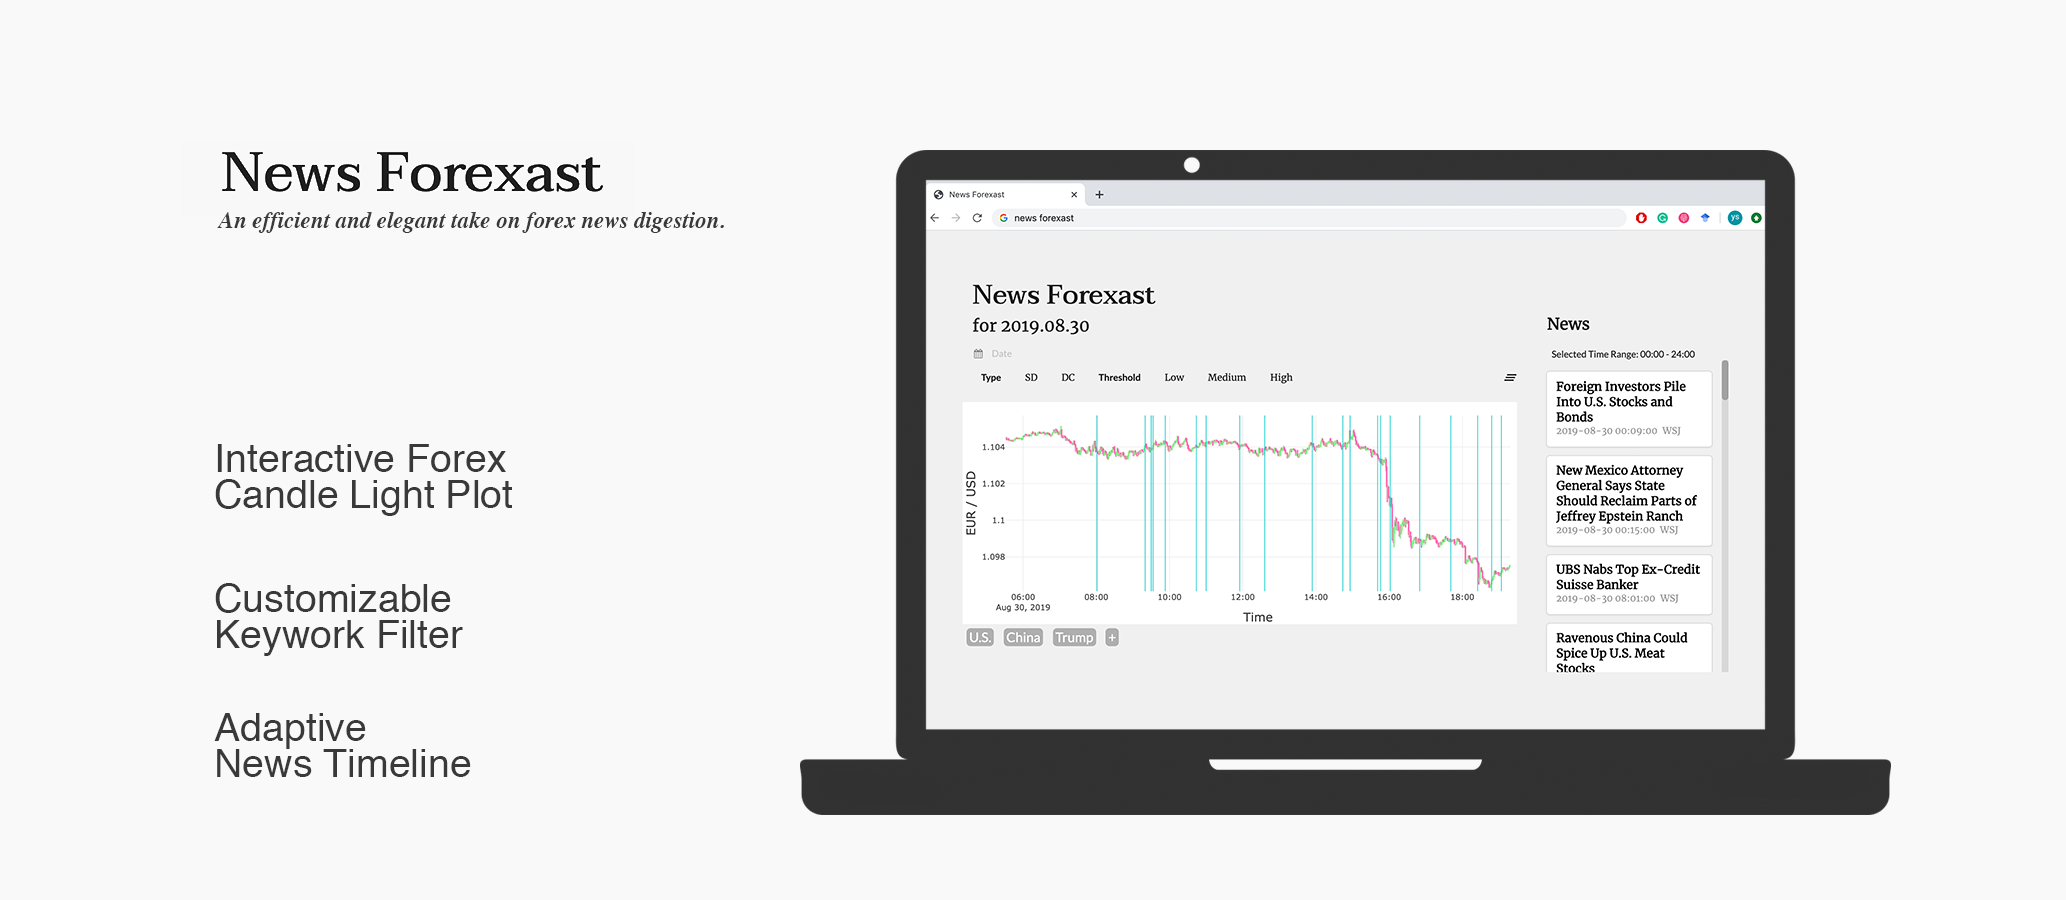
\includegraphics[width=\textwidth]{teaser.png}
  \caption{Forexast available at http://}
  \Description{}
  \label{fig:teaser}
\end{teaserfigure}


%%
%% This command processes the author and affiliation and title
%% information and builds the first part of the formatted document.
\maketitle

\section{Introduction}
Foreign exchange (Forex) market has been one of the most popular financial markets for decades, with an estimated \$1\ trillion traded every day~\cite{YAO200079}.
Spot trading, currency options, currency futures, and currency exchange-traded funds (ETFs) are four major ways to trade Forex~\cite{TradeForex}.
The strategies might vary but they are driven by an intuitive rule of thumb, which is to buy low and sell high~\cite{KOOLEN2014144,Zervos11}.
Therefore, whether investors can accurately forecast the prices or trends is extremely crucial. 

Forex markets are influenced by numerous factors, such as producer price index (PPI), interest rates, and politics.
In order to consider as many factors as possible to have more comprehensive views for Forex investment, most investors rely on news for them to stay informed.
Besides the fact that news usually reflect the real-world events, the similar nature of news and forex also makes these two co-dependent.
For example, if the Federal Reserve System (Fed) cuts the interest rate, it is more likely that the value of USD would drop; also, such a devaluation would later make another piece of news~\cite{"CNBC"}. 

Considering the critical roles of news for Forex investment, in this demonstration, we propose Forexast, an interactive web-based system that displays a forex plot alongside with related financial news.
The proposed system aims to highlight the connection between two types of time-series data: the Forex and the news data by aligning the timing of them.
Forexast is designed to display the news' release time as vertical lines on the forex plot to emphasize the order of breaking news and exchange rates. In addition, when users hover on a vertical line, the background colour of the corresponding news would change. 
Moreover, we propose to use two event detection methods based on the standard deviation (SD) and directional change (DC)~\cite{7850020} of the Forex data to locate specific periods when the trends in Forex markets dramatically change.
Via this design, user can pay more attention to the changes of trend or where the prices have larger volatility.
Finally, Forexast comes with a keyword filtering function that allows users to filter news with self-defined keywords.
To our best knowledge, this is the first system that effectively visualizes two types of time-series data: the forex data and the textual news data in a unified and time-aware manner. 
The proposed Forexast can be of great help in revealing valuable insights and relations between two types of time-series data and thus be valuable for decision making for not only professional financial analysts or 

The remainder of this paper is organized as follows.
In Section~\ref{sec:related}, we review previous studies related to Forex and news and major websites for Forex traders.
Section~\ref{sec:system} describes the proposed system with details related to data collection, event detection algorithms, interfaces and key features.
After that, we provide a case study in section~\ref{sec:case} and Section~\ref{sec:conclude} provides the conclusion and future work.

\section{Related Work and Systems}\label{sec:related}
The dynamics between news and Forex markets have been explored from several different aspects.
Evans and Lyons (2005) prove that news can have significant effects on currency for days~\cite{EVANS2005197}, and macro news can affect currency prices directly and indirectly via order flow~\cite{EVANS200826}.
There is also more evidence showcasing news and Forex trend are correlated.
For instance, Bauwens et al.  (2005) show that volatility increases right before the announcement of scheduled news and unscheduled-but-periodic news~\cite{BAUWENS20051108}, while Chatrath et al. (2014) suggest that prices respond quickly within 5-min after the news release~\cite{CHATRATH201442}.
With how Forex markets and news interact in mind, it is reasonable for traders to begin their days by reading news commentary to determine the market sentiment and the direction for trading~\cite{samuels2015trader}.

Apart from the literature discussing the relation between Forex and news, there are many trading websites which provide useful information for Forex investors, each of which has its own features and limitations~\cite{ForexWebsites}.
For instance, BabyPips\footnote{\url{https://www.babypips.com}} is a friendly website for junior traders, providing not only Forex plots but also courses, tutorials and forums for beginners. Bloomberg\footnote{\url{https://www.bloomberg.com}} is a well-known news agency; thus, in addition to currency data and plots, it also provides various categories of news for users to focus on their interest.
TradingView\footnote{\url{https://www.tradingview.com}} provides numerous functions in a page, such as watchlist, alerts, headlines and real-time chats, where users can customize the settings. 
However, most of these websites do not put the news and Forex plot at the same page or do not explicitly align the news releasing time with the Forex prices.
Most of them neglect the time-dependent relation between news and Forex data and thus do not effectively visualizes two types of time-series data: in a unified and time-aware manner. 


\section{System Description}\label{sec:system}

\subsection{Data Collection}
The forex data is from philipperemy/FX-1-Minute-Data\footnote{\url{https://github.com/philipperemy/FX-1-Minute-Data}}, a repository of github. We choose the EUR/USD index, and use the DateTime Stamp, OPEN Bid Quote, HIGH Bid Quote, LOW Bid Quote and CLOSE Bid Quote columns as our forex data. The time span is from 2019/08/04 to 2019/09/13 except Saturdays, and the granularity of data is minute. 

The news data is crawled by us, containing titles, sources, release times and urls. There are 1116 news in total and the sources are all from The Wall Street Journal\footnote{\url{https://www.wsj.com}}.

\subsection{Algorithms for SD and DC events}
To mark some special time points on the plot, we use two algorithms, standard deviation events (SD events) and directional change events (DC events)\cite{7850020}. SD events show the times where the prices dramatically change, and DC events show the times where the trends change. To get these events, we need to calculate the difference rate list $D$ of the price list first. 
Let $P= [p_1, p_2, ..., p_n]$, where $p_t$ stands for the CLOSE Bid Quote at minute $t$ and n equals to total numbers of daily forex data. Then we can get a difference rate list $D= [d_1, d_2, ..., d_m]$, where $d_t = \frac{p_{t+w}-p_t}{p_t}$.  $w\in\mathbb Z^+$ means the range in minutes, which can be freely customized (we use 30 in this demonstration).
$\sigma$ is the standard deviation of $D$, which can be interpreted as the volatility of prices. We use $\sigma$ as our low threshold to attain a subset of D, whose elements are all bigger than $\sigma$. Then the corresponding set of p will be marked as SD events. We also consider $2\sigma$ and $3\sigma$ as medium and high thresholds in our demonstration. Higher threshold will find less events.

Under the DC framework, the market is summarized into alternating uptrends and downtrends\cite{7850020}. A DC event, including a start point and an end point, can be seen as a period that the trend starts to change. At first, we do not know the prices start with a upward or downward trend, so we let the first element of price $p_1$ as a base. Then we start looking through the list until we find a current price $p_c$, where $|\frac{p_c-p_1}{p_1}| > \theta$, $\theta$ can be set to $\sigma$, $2\sigma$, $3\sigma$ as above mentioned. If $p_c > p_1$, that means the span from $p_1$ to $p_c$ is an upward DC event; otherwise, it is a downward DC event. After finding the first DC event, we still have to look through the rest. Let us consider a market starts with a downtrend, which means we are now in an downtrend and waiting for a next uptrend. We keep updating the lowest price $p_l$ in this downtrend until we find a current price $p_c$ that $\frac{p_c-p_l}{p_l} > \theta$. Then, we mark that the span from $p_l$ to $p_c$ is a upward DC event, and the trend become upward. Similarly, if a market is in a uptrend, we keep updating the highest price $p_h$ until we find a current $p_c$ that $\frac{p_h-p_c}{p_c} > \theta$, then $p_h$ to $p_c$ is a downward DC event, and the trend become downward. After finishing looking through all daily forex data, we can get a series of alternating DC events.




\subsection{Interfaces and features}
The interface of News Forexast can be divided into two main parts, a forex chart and the news section. Users can customize the selection criteria either by directly manipulating the forex chart or applying the keyword filters.

\begin{figure}[h]
  \centering
  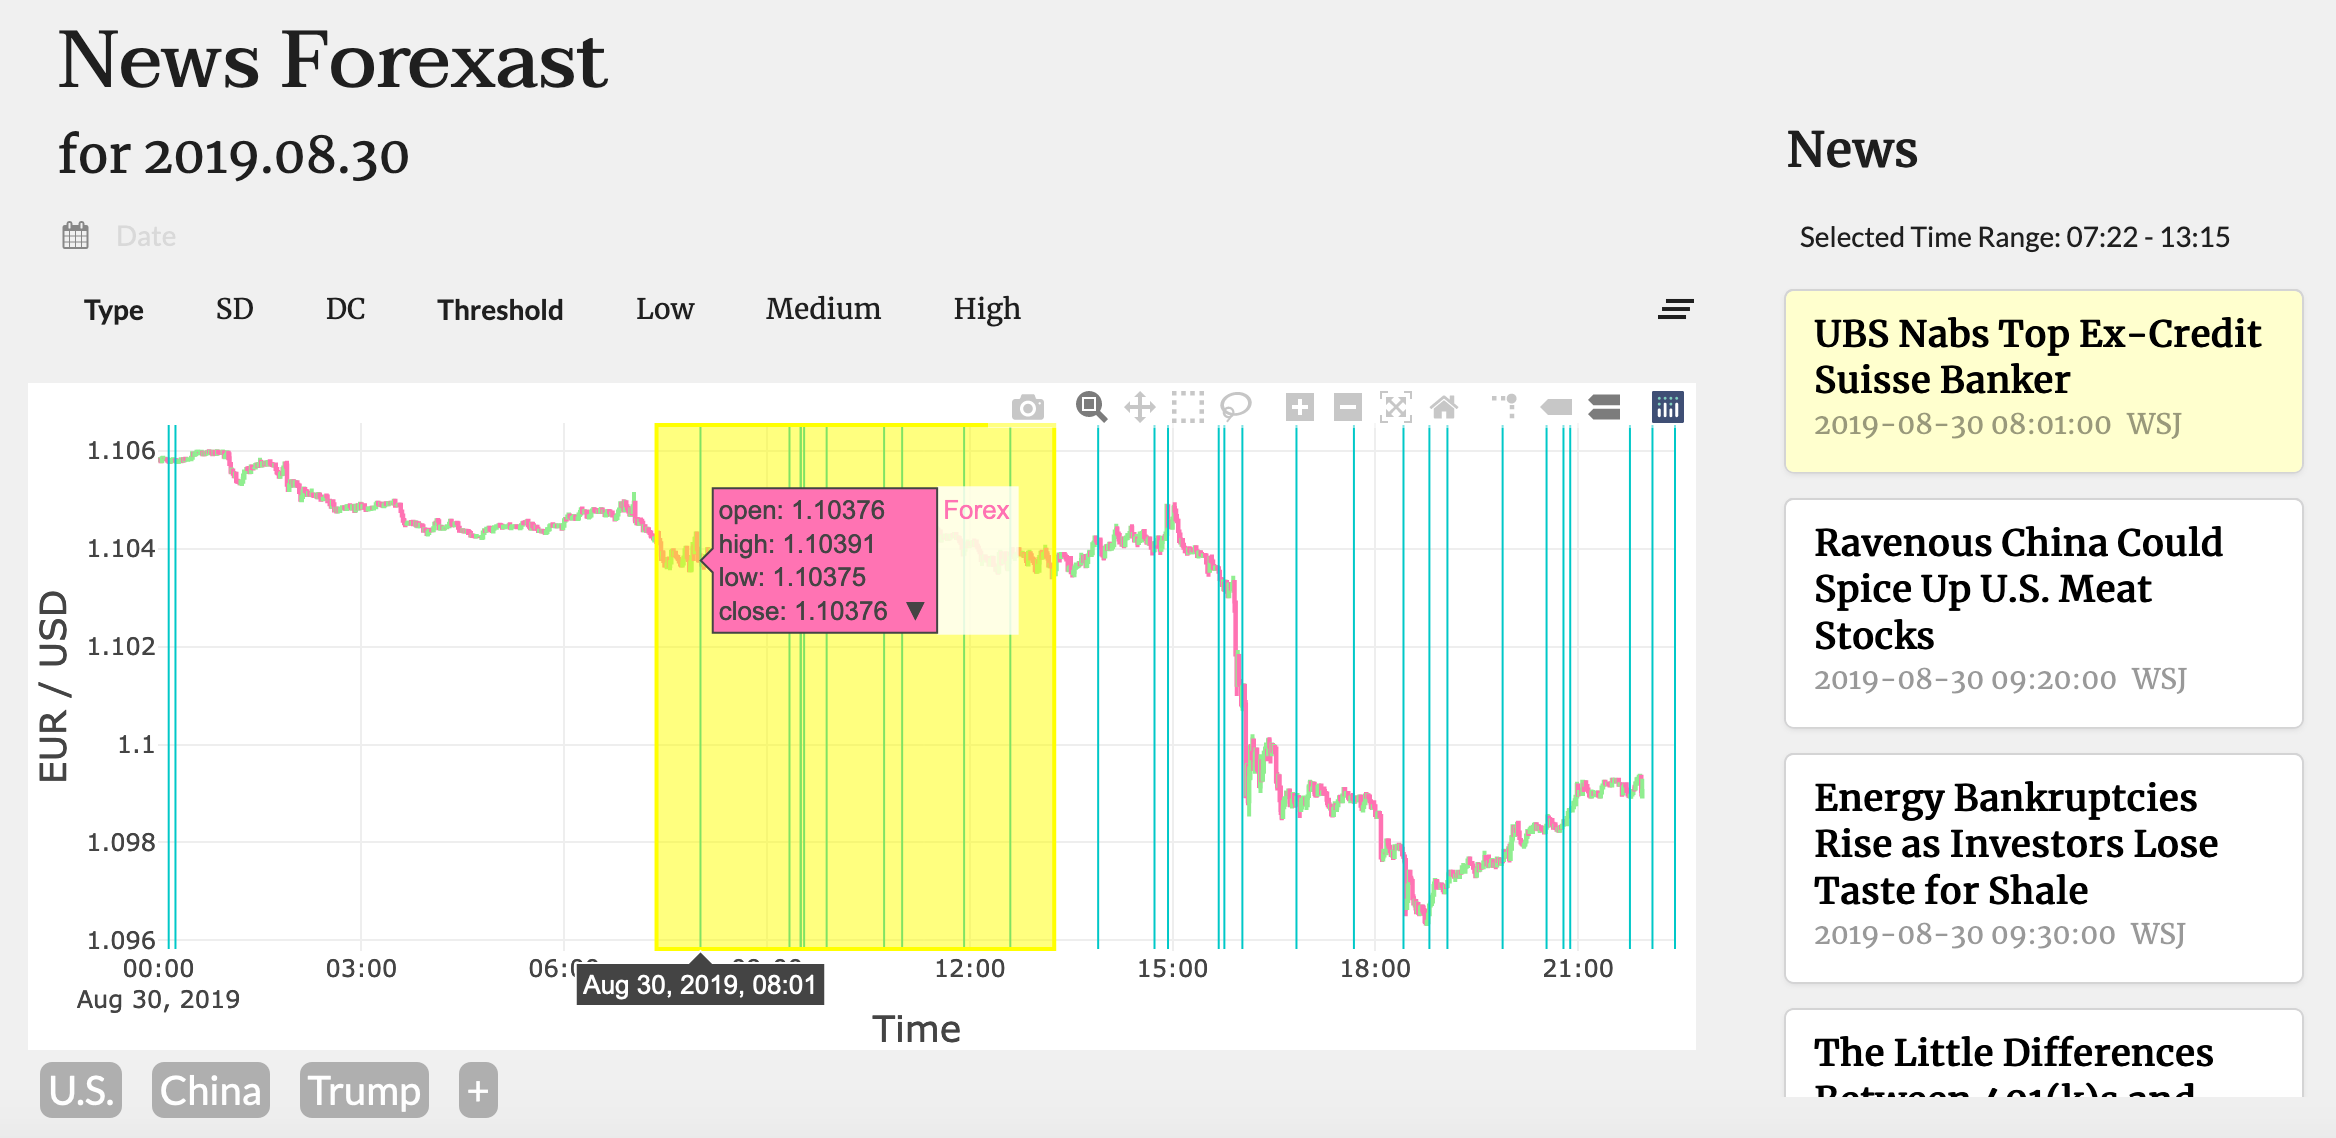
\includegraphics[width=\linewidth]{hover.png}
  \caption{Example of news being highlighted when the cursor hovers over the corresponding timeline on the chart. The yellow interval is the news selection range which can be decided by users.}
  \Description{}
\end{figure}

\subsubsection{Interactive Forex Chart}
The forex chart is a standard candlestick chart, powered by Plotly graphing libraries\footnote{\url{https://https://plotly.com/graphing-libraries/}}, that displays price movements, users can specify the date they are interested in with the calendar icon above the chart. Supported by Plotly graphing library, users can explore the chart freely by zooming in or dragging out the time frame they are interested. The corresponding news would be highlighted if users hover over the corresponding blue line on the chart. (Fig. 2)


Below the calendar is where users can specify event types and the corresponding thresholds. After selecting an event type and their thresholds, eg. SD and low threshold,  the algorithmic output would be shown on the forex chart. Once done with a specific setting, users can clear the setting with the “clear all” button the top-right. The news section without any specification would show all daily news with titles, released time and sources. Users could link to the original posts and websites by clicking on the news cards. 



\subsubsection{Forex Event Identifier}
With the help of SD and DC events as indicators, users can now spot specific time ranges they are interested in. (Fig 3, 4) Users can then select such time range on the plot and narrow down the news shown on the right to the time range they selected. For example, users can specify 2019/08/30 with the SD with the low threshold, users can tell that there’s a dramatic change during 14:30-16:30 and can proceed to select the time range on the plot. In return, the news section would display related news such as "Would Warren Buffett Buy Greenland?" and "Risky Seller Financing Flourishes Where Homes Are Cheapest". 

\begin{figure}[h]
  \centering
  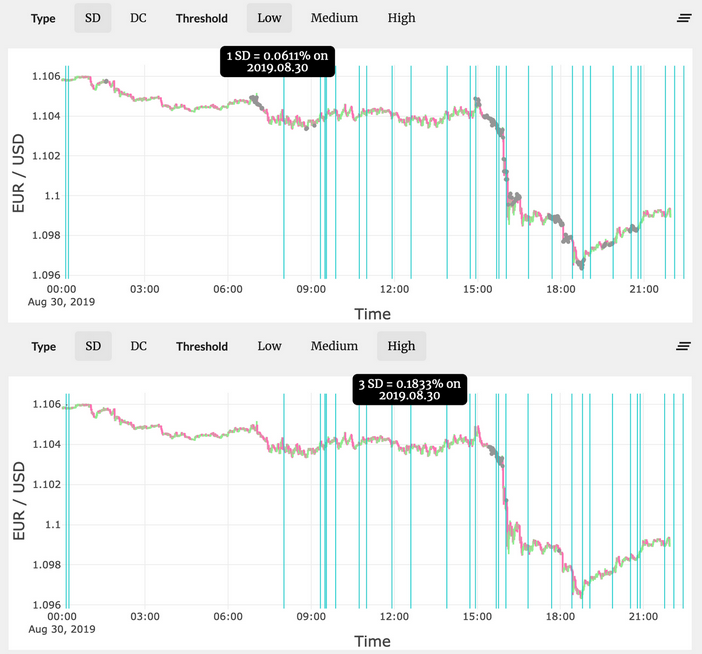
\includegraphics[width=\linewidth]{sd.png}
  \caption{Examples of displaying SD events on 2019/08/30. The top is set to low threshold and the bottom is set to high threshold. Due to the higher sensitivity, almost all events of the latter are in the slump period around 16:00.}
  \Description{}
\end{figure}

\begin{figure}[h]
  \centering
  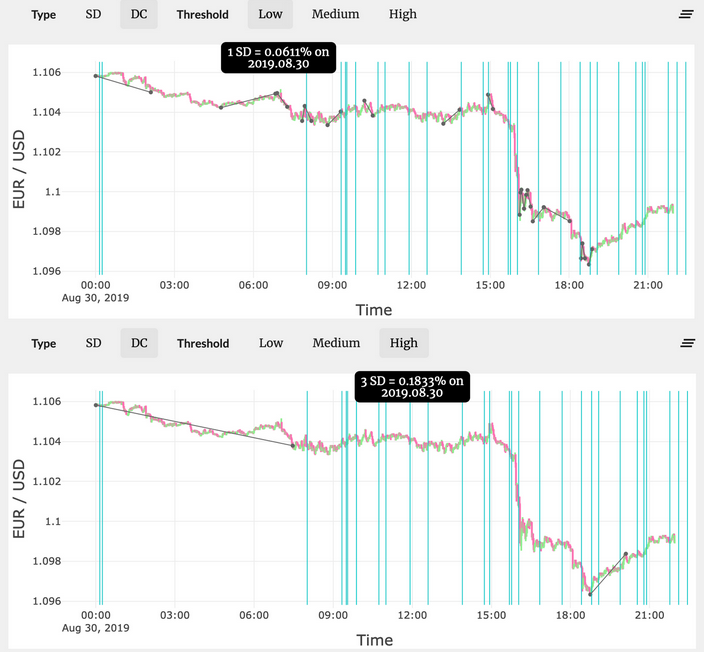
\includegraphics[width=\linewidth]{dc.png}
  \caption{Examples of displaying DC events on 2019/08/30. The top is set to low threshold and the bottom is set to high threshold. Due to the higher sensitivity, the latter only summarize the daily market into a downtrend and an uptrend.}
  \Description{}
\end{figure}

\subsubsection{Customizable Keyword Filter
}
If interested in more specific news, users can use the button under the plot to filter out news with selected keywords. We have placed several keywords such as U.S. and Trump, users can also customize their own tags by clicking the “+” button. For example, if the time frame is specified and the tag "U.S" is applied, only "Strength in U.S. Consumer Spending Drives Economy". would be shown on the news section.(Fig 5)


\begin{figure}[h]
  \centering
  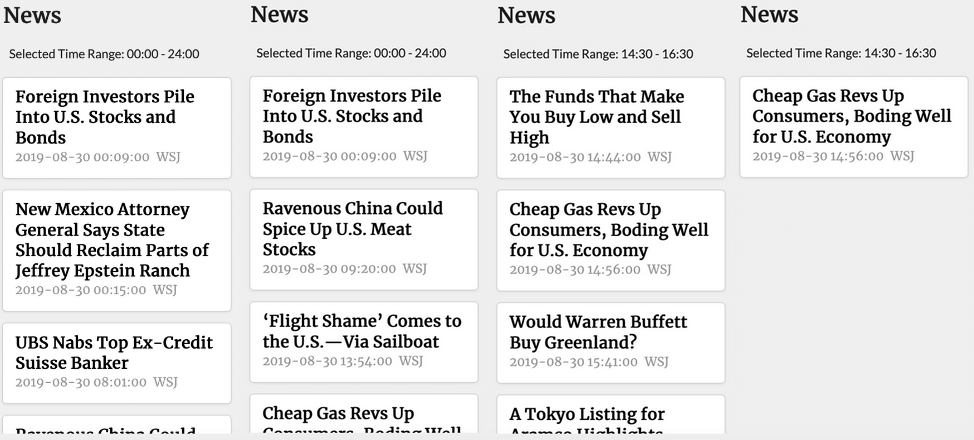
\includegraphics[width=\linewidth]{news.png}
  \caption{Examples of filtering news on 2019/08/30. From left to right are none, keyword: 'U.S.', time: '14:30-16:30', and both.}
  \Description{}
\end{figure}

\section{Case Study}\label{sec:case}

\begin{figure}[h]
  \centering
  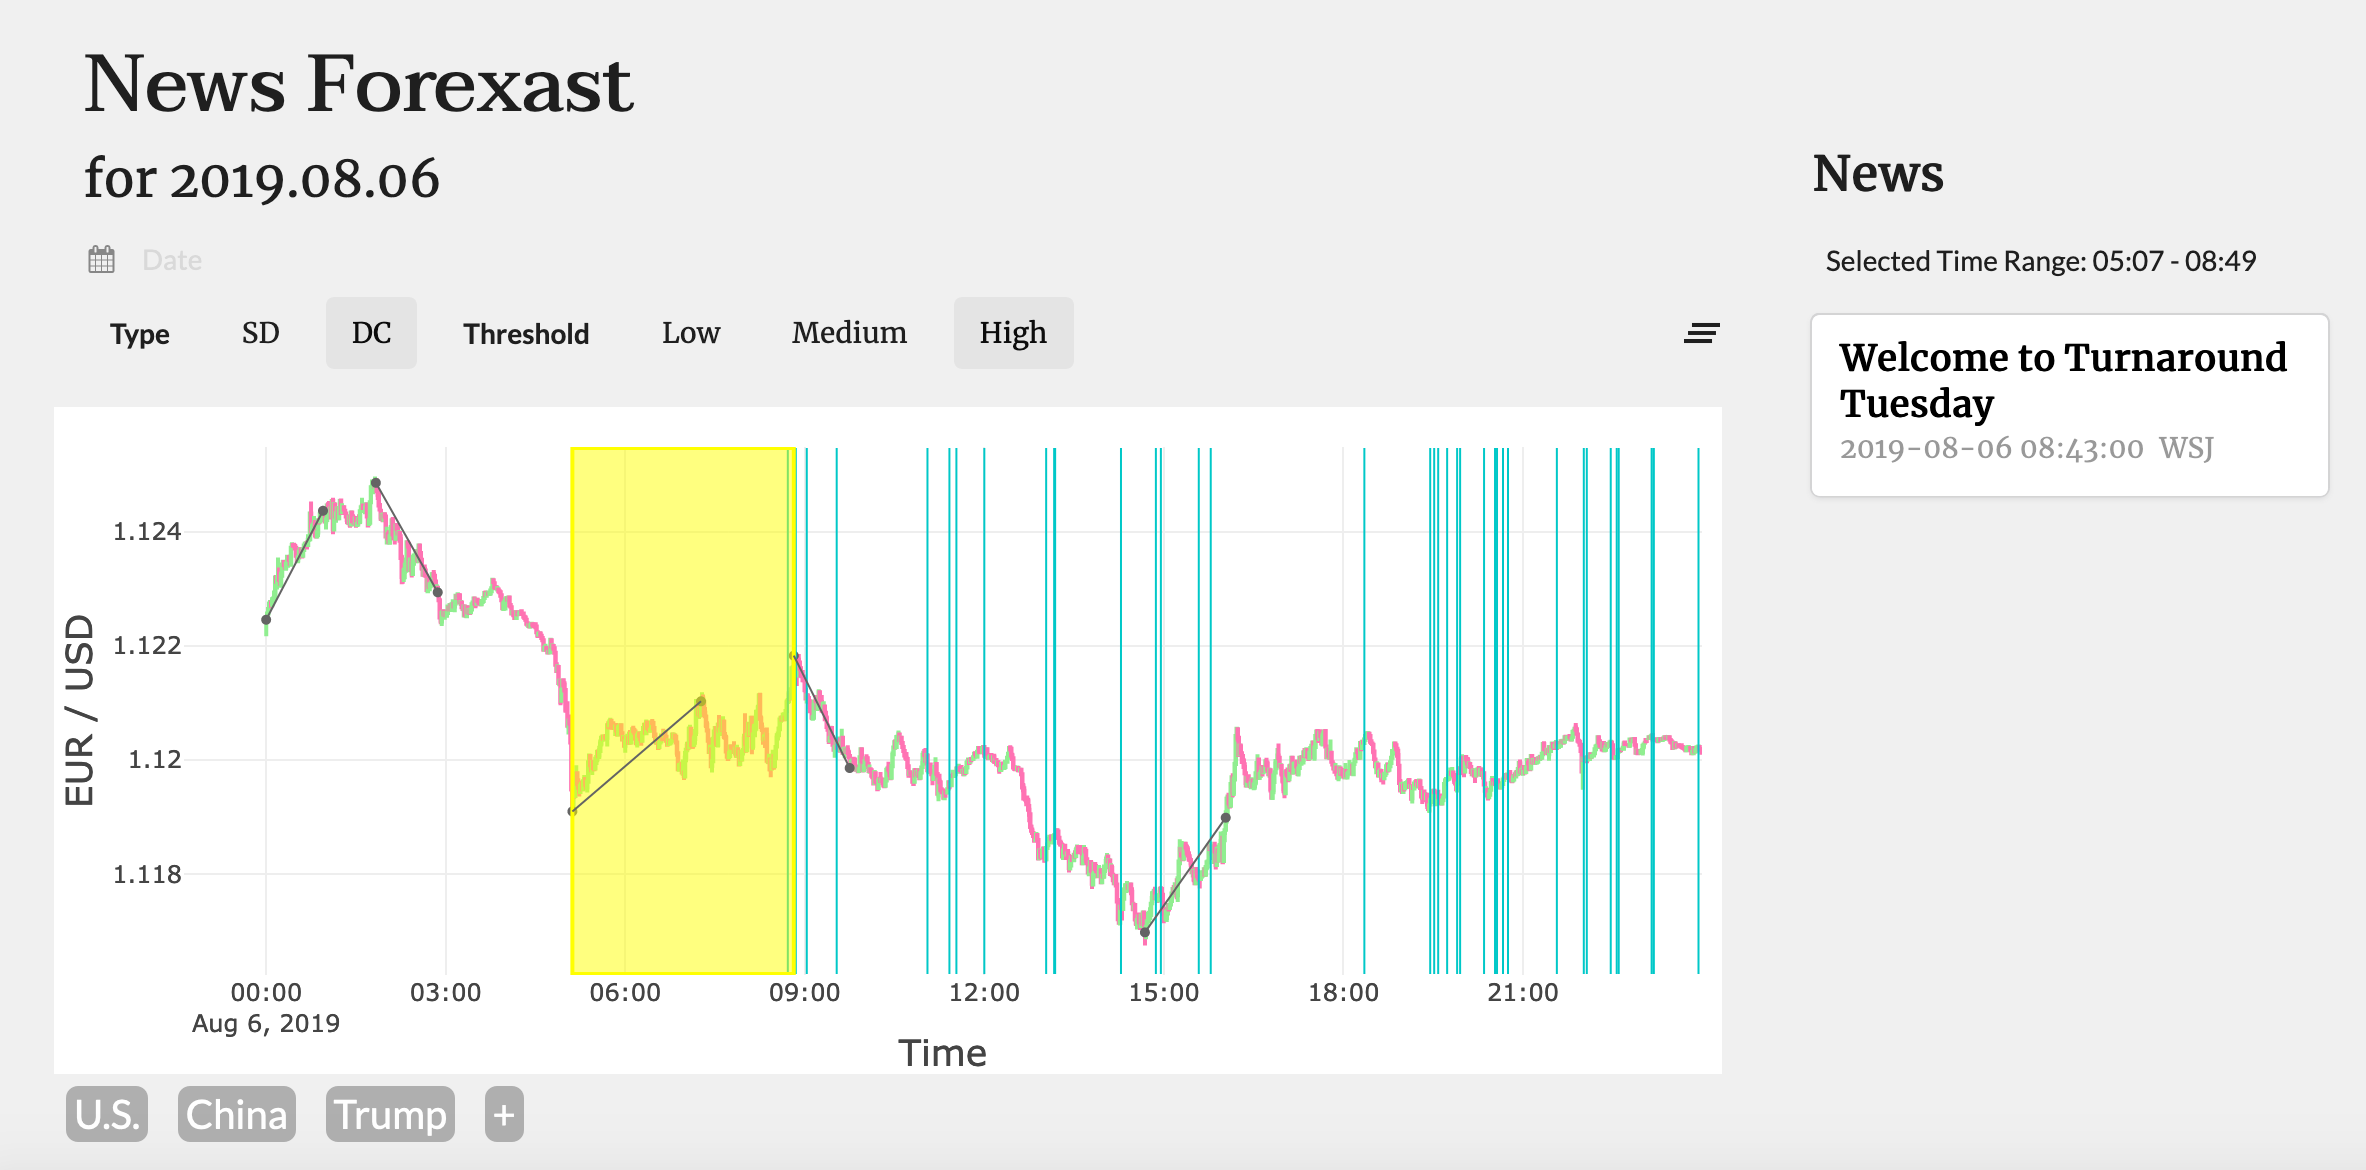
\includegraphics[width=\linewidth]{case.png}
  \caption{An example of case study.}
  \Description{}
\end{figure}

In this section, we provide an example that showcases the strong relation among events, news and forex (Fig 6). On 2019/08/06, we can see the news "Welcome to Turnaround Tuesday" released at 08:43, the time when an uptrend is about to end (displaying DC event with high threshold shows that this uptrend starts at 05:07). The news mentioned "U.S. stock futures were in a decidedly better mood as Tuesday began than on Monday." This indicates that U.S. stock is likely to rebound later, and thus causes appreciation on USD. Then, the EUR/USD starts a downtrend from 08:49 to 14:41. Note that if EUR/USD has lower rate, it could be explained that USD has relatively high value.



\section{Conclusion and Future work}\label{sec:conclude}
We have proposed an interactive website that juxtaposes a forex chart with news from the time frame users selecting. By having the chart and related news side by side together, users, financial professional or amateur investors, can all understand the trend quicker and easier. We are working toward to provide real-time news update in the future, as forex data is limited. In addition, if we are able to collect more user's log data and news in the future, along with machine learning and natural language processing (NLP) techniques, we can achieve more customized news feed such as personal news recommendation.  

\section{Acknowledgments}



\bibliographystyle{ACM-Reference-Format}
\bibliography{reference}




\end{document}
\endinput
%%
%% End of file `sample-sigconf.tex'.
